\chapter{Réalisation et Implémentation}
\label{chap:implementation}

\section{Introduction}

\par Après avoir présenté l'analyse des besoins ainsi que la conception de l'application TuniPark, ce chapitre décrit la phase de réalisation du projet. Il présente les principaux outils utilisés durant le développement ainsi que l'implémentation des différents modules constituant la solution.

\par Le chapitre présente tout d'abord l'environnement de développement adopté, puis décrit l'implémentation du Backend, de l'application mobile Flutter, de la plateforme web d'administration Angular, ainsi que l'intégration des différents services externes. Enfin, il présente le système de recommandation intelligent ainsi que les principales fonctionnalités développées.


\section{Environnement de développement}

\par La réalisation de l'application \textbf{TuniPark} a nécessité l'utilisation de plusieurs outils et technologies couvrant le développement mobile, le développement web, le développement Backend, l'IA, la gestion de la base de données, les tests, le déploiement tout comme l'intégration de différents services externes. Ces technologies ont été sélectionnées afin de garantir une architecture moderne, performante et facilement maintenable.

\begin{table}[H]
\centering
\small
\renewcommand{\arraystretch}{1.25}
\begin{tabular}{|p{0.32\textwidth}|p{0.58\textwidth}|}
\hline
\textbf{Outil / Technologie} & \textbf{Mise en œuvre dans le projet} \\
\hline
\textbf{Flutter} & Réalisation de l'application mobile destinée aux utilisateurs. \\
\hline
\textbf{Angular} & Élaboration de la plateforme en ligne d'administration. \\
\hline
\textbf{NestJS} & Développement de l'API Backend et de la logique métier. \\
\hline
\textbf{Prisma ORM} & Couche d'accès aux données et gestion des modèles PostgreSQL. \\
\hline
\textbf{PostgreSQL} & Stockage des données de l'application (utilisateurs, parkings, sessions, paiements, notifications, etc.). \\
\hline
\textbf{Python FastAPI} & Développement du microservice d'IA utilisé pour la recommandation des parkings. \\
\hline
\textbf{Scikit-learn (Random Forest)} & Implémentation du modèle de recommandation intelligent. \\
\hline
\textbf{Cloudinary} & Stockage et gestion des images des parkings. \\
\hline
\textbf{Firebase Cloud Messaging} & Envoi des notifications Push vers les appareils mobiles. \\
\hline
\textbf{Flouci} & Gestion des paiements électroniques des sessions de stationnement. \\
\hline
\textbf{Nodemailer} & Envoi des courriers électroniques (vérification et récupération de compte). \\
\hline
\textbf{Twilio} & Gestion des codes OTP par SMS (prévu, non activé durant le projet). \\
\hline
\textbf{Postman} & Test et validation des services REST du Backend. \\
\hline
\textbf{Render} & Plateforme utilisée pour héberger le Backend NestJS, le microservice IA basé sur FastAPI, ainsi que la base de données PostgreSQL. \\
\hline
\textbf{Vercel} & Hébergement de la plateforme web d'administration Angular. \\
\hline
\textbf{Git \& GitHub} & Gestion des versions et collaboration durant le développement. \\
\hline
\end{tabular}
\caption{Principaux outils et technologies utilisés lors de l'implémentation de TuniPark}
\label{tab:implementation_tools}
\end{table}
\section{Implémentation du Backend}

\par Le Backend de \textbf{TuniPark} a été développé à l'aide du framework \textbf{NestJS}. Il constitue le cœur de l'application en assurant le traitement des requêtes provenant de l'application mobile Flutter et de la plateforme web d'administration Angular. Il applique les règles métier, communique avec la base de données PostgreSQL via Prisma ORM et interagit avec plusieurs services externes tels que Flouci, Firebase Cloud Messaging, Cloudinary, Nodemailer ainsi que le microservice d'IA.

\par Afin de garantir une architecture claire, évolutive et facilement maintenable, le Backend est organisé suivant une architecture modulaire. Chaque module est responsable d'un domaine fonctionnel spécifique, ce qui facilite le développement, les tests unitaires et l'évolution future de l'application.
\subsection{Module d'authentification}

\par Le module d'authentification assure la sécurisation de l'accès à l'application. Il prend en charge l'inscription, la connexion, le renouvellement des sessions ainsi que la récupération de mot de passe.

\par Suite à une authentification réussie, le Backend produit un jeton d'accès et un jeton de renouvellement basés sur JWT. Les accès aux différentes fonctionnalités sont ensuite contrôlés en fonction du rôle de l'utilisateur (\textit{Utilisateur}, \textit{Administrateur}, \textit{Propriétaire de parking} ou \textit{Auditeur}). Le module intègre également la vérification des adresses électroniques via Nodemailer ainsi que la vérification des numéros de téléphone par code OTP.

\begin{figure}[H]
    \centering
    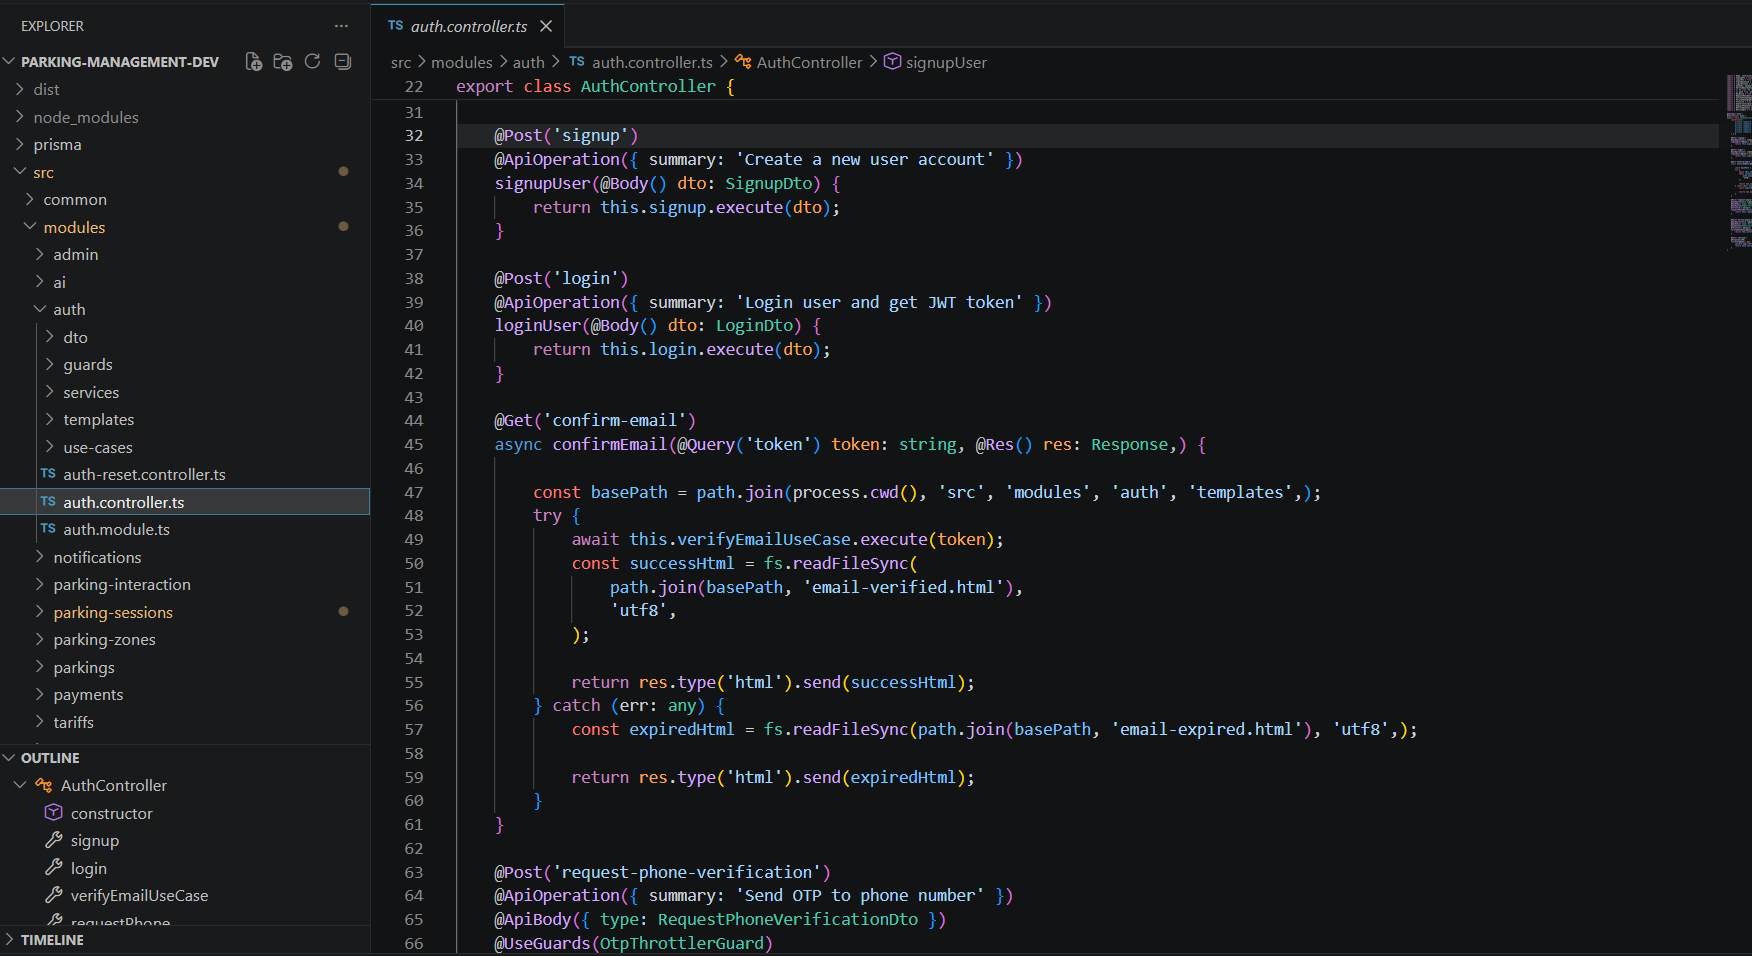
\includegraphics[width=\textwidth]{img/backend_auth.png}
    \caption{Implémentation du module d'authentification}
    \label{fig:backend_auth}
\end{figure}
\subsection{Module de gestion des parkings}

\par Ce module permet la création, la modification et la gestion des parkings publics et privés. Les propriétaires peuvent publier un nouveau parking en renseignant ses caractéristiques, sa localisation, sa capacité, ses horaires, son tarif ainsi que les images correspondantes.

\par Les images sont automatiquement téléversées sur Cloudinary tandis que les informations descriptives sont enregistrées dans PostgreSQL. Les parkings privés sont initialement enregistrés avec le statut \texttt{PENDING} avant d'être validés ou rejetés par un administrateur.

\begin{figure}[H]
    \centering
    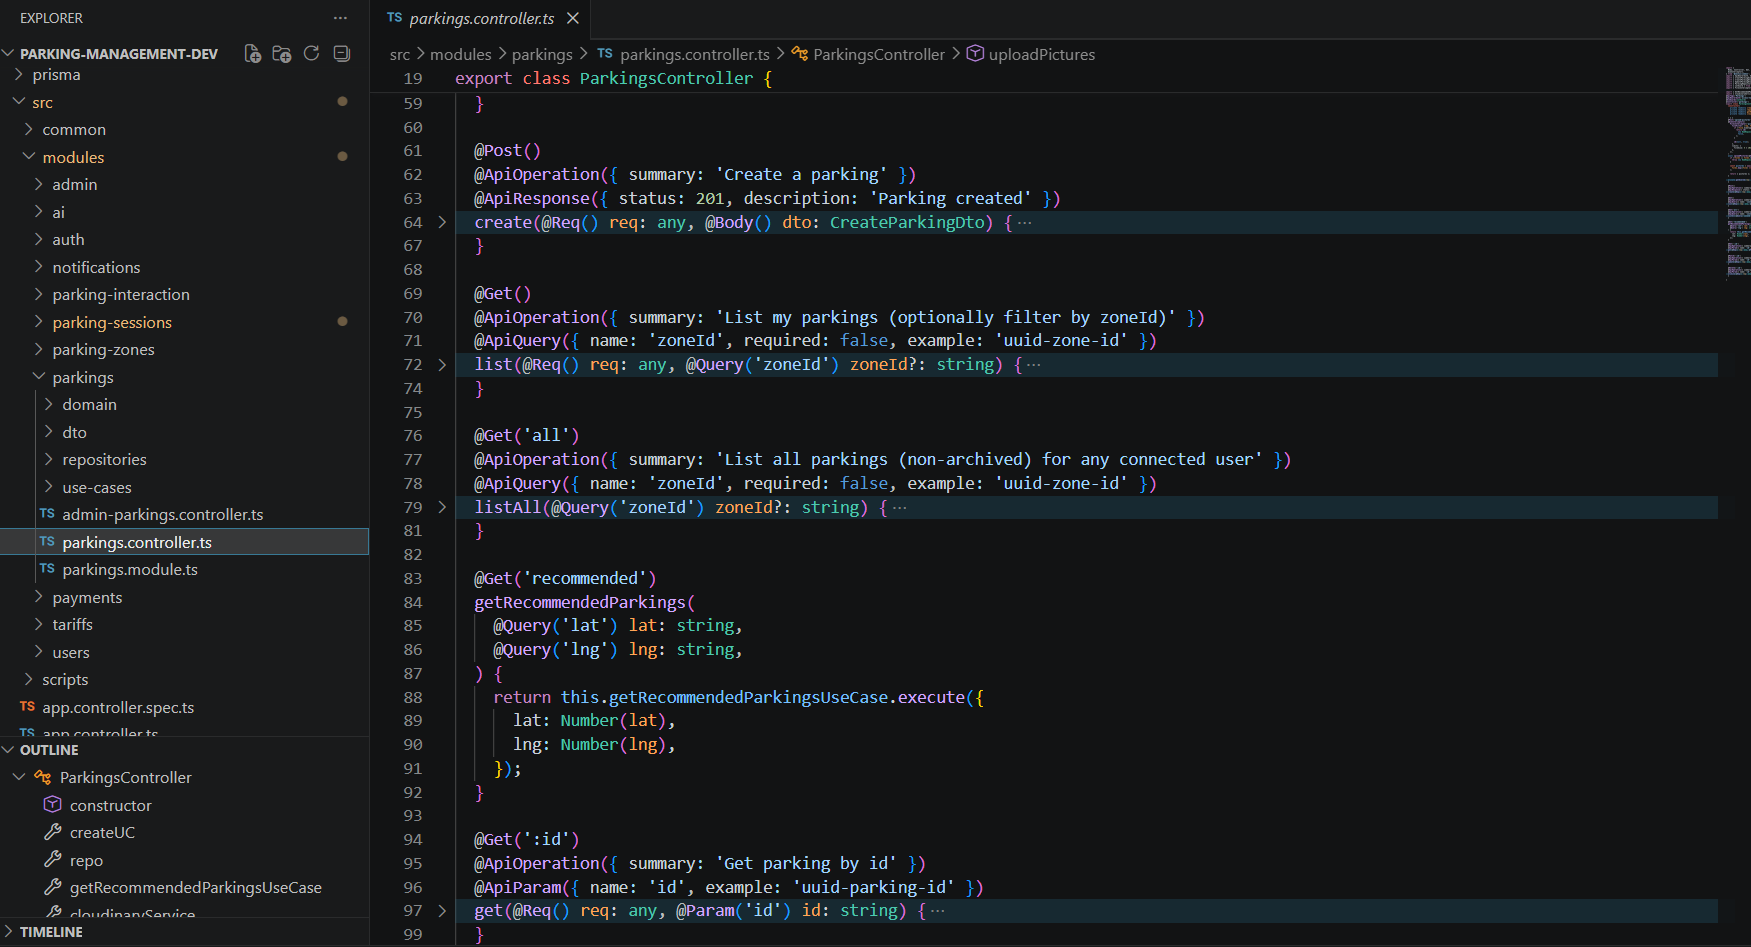
\includegraphics[width=\textwidth]{img/backend_parking.png}
    \caption{Implémentation du module de gestion des parkings}
    \label{fig:backend_parking}
\end{figure}

\subsection{Module de gestion des tarifs}

\par Le module de gestion des tarifs permet d'associer une grille tarifaire à chaque parking. Il prend en charge les différents modes de facturation proposés par la plateforme, notamment le tarif à l'unité, le tarif journalier et le tarif mensuel.

\par Les administrateurs et les propriétaires de parkings peuvent définir ou modifier les tarifs en fonction des caractéristiques de chaque parking. Ces informations sont utilisées lors de la création des sessions de stationnement afin de calculer le montant à payer par l'utilisateur.

\begin{figure}[H]
    \centering
    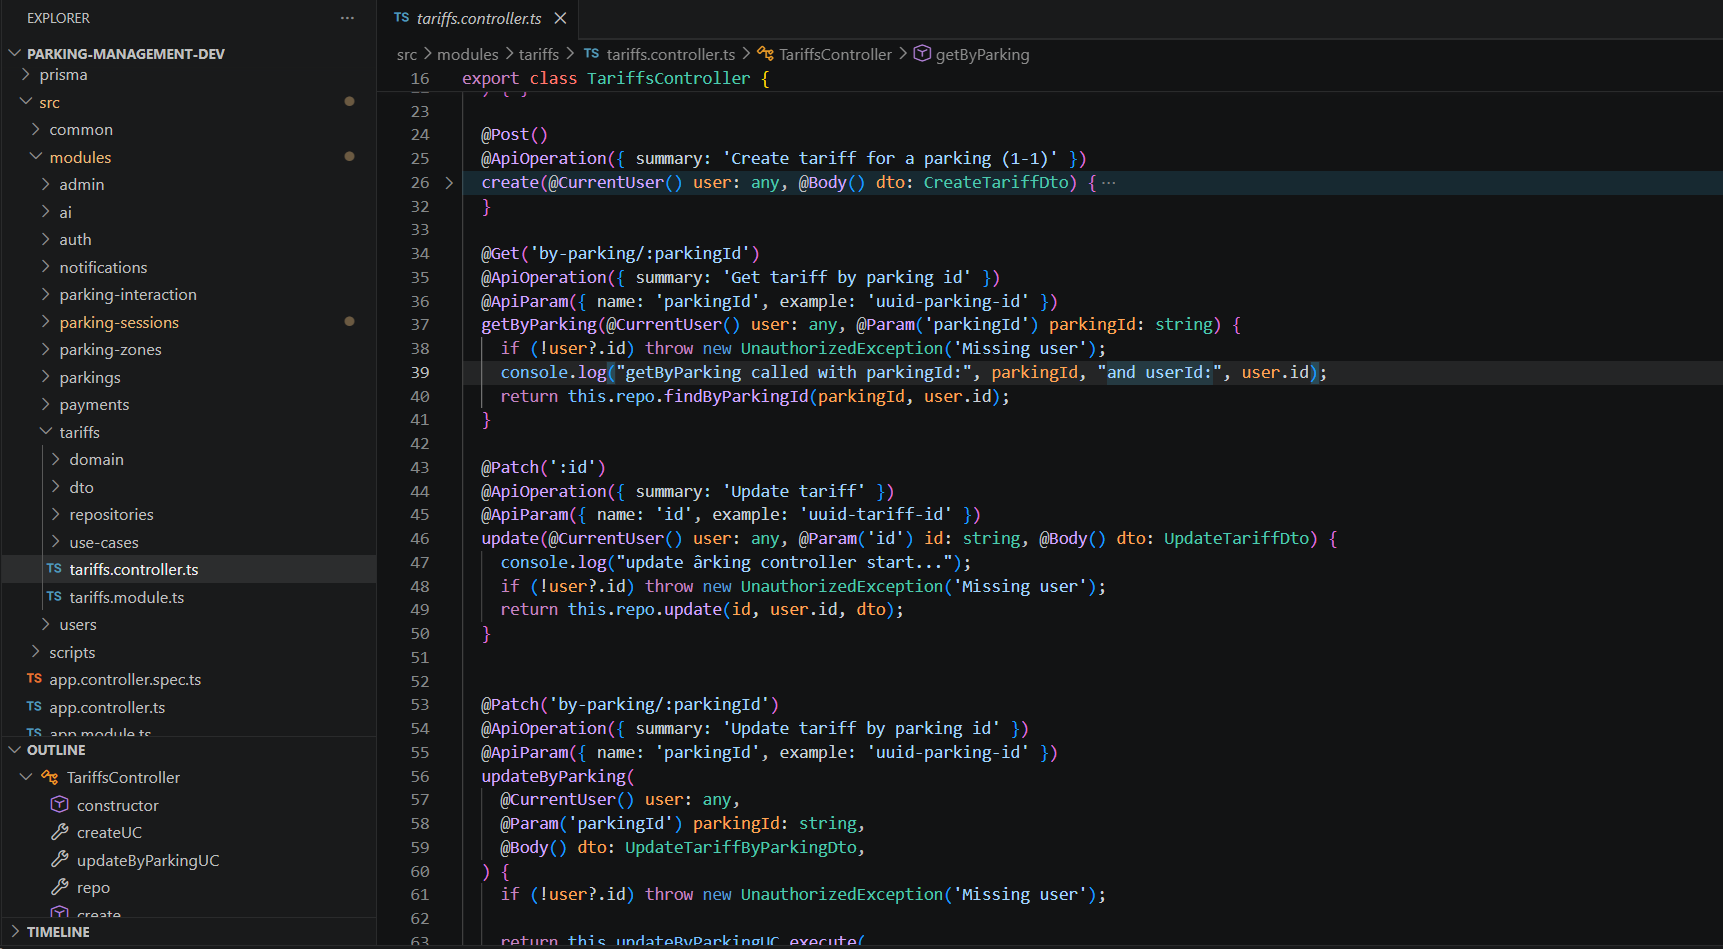
\includegraphics[width=\textwidth]{img/backend_tariff.png}
    \caption{Implémentation du module de gestion des tarifs}
    \label{fig:backend_tariff}
\end{figure}

\subsection{Module de gestion des sessions de stationnement}

\par Le module des sessions permet aux utilisateurs de démarrer, prolonger et terminer une session de stationnement. Lorsqu'un utilisateur sélectionne un parking, le Backend vérifie sa disponibilité avant de créer une nouvelle session avec le statut \texttt{CREATED}.

\par Après validation du paiement, le statut de la session devient \texttt{ACTIVE}. Le module assure également le suivi des différentes étapes du stationnement jusqu'à la fermeture de la session, tout en conservant l'historique des opérations.

\begin{figure}[H]
    \centering
    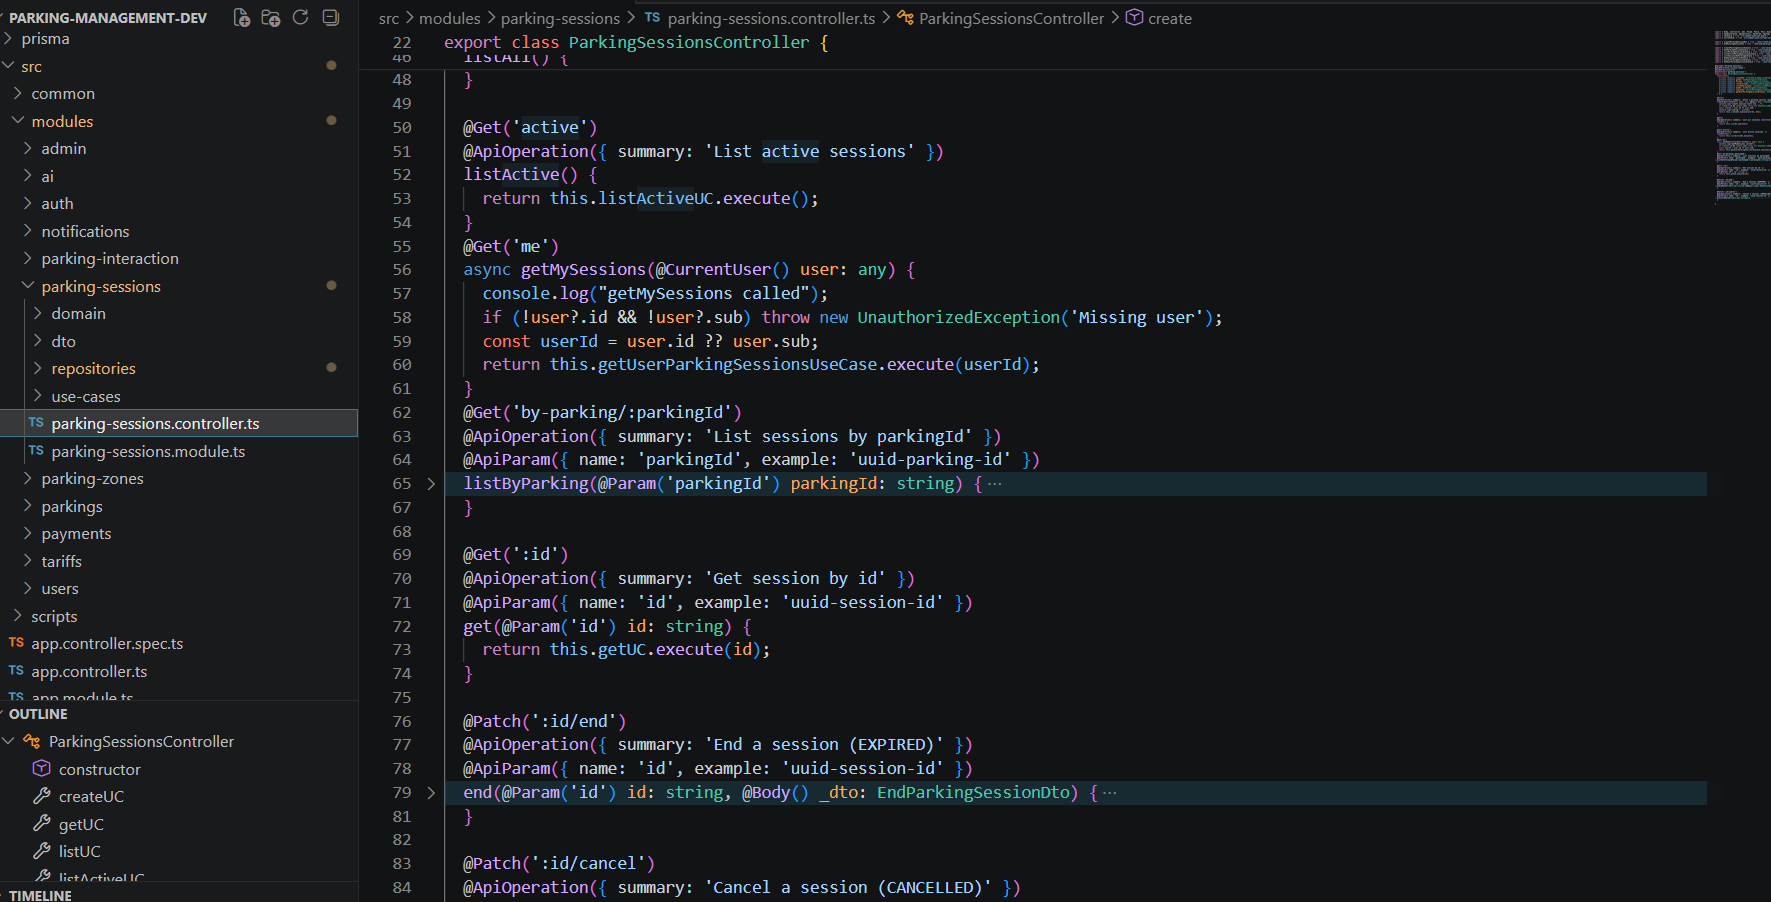
\includegraphics[width=\textwidth]{img/backend_session.png}
    \caption{Implémentation du module des sessions de stationnement}
    \label{fig:backend_session}
\end{figure}

\subsection{Module de paiement}

\par Le module de paiement permet de gérer les transactions financières liées aux sessions de stationnement. Après la création d'une session, le Backend prépare automatiquement la transaction puis redirige l'utilisateur vers la plateforme de paiement \textbf{Flouci}.

\par Une fois le paiement confirmé, Flouci informe le Backend du résultat de la transaction. Celui-ci met alors à jour les informations de paiement ainsi que le statut de la session. Toutes les transactions sont enregistrées dans la base de données afin d'assurer leur traçabilité.

\begin{figure}[H]
    \centering
    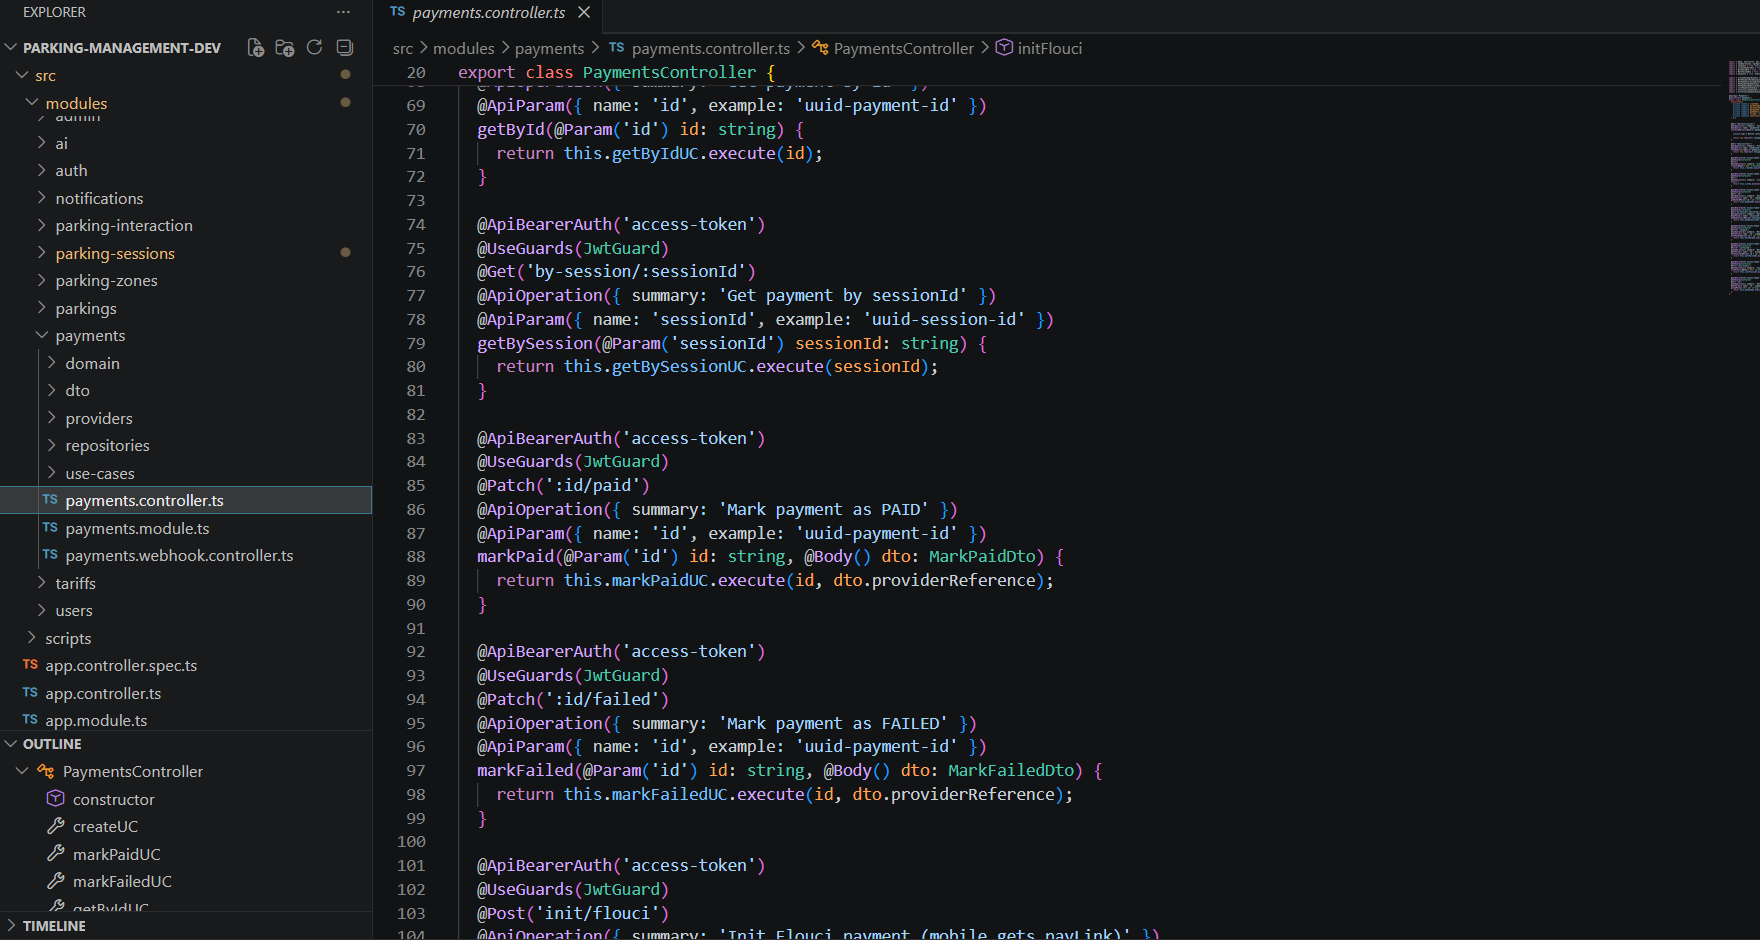
\includegraphics[width=\textwidth]{img/backend_payment.png}
    \caption{Implémentation du module de paiement}
    \label{fig:backend_payment}
\end{figure}
\subsection{Module de recommandation intelligente}

\par Pour offrir une meilleure expérience aux utilisateurs, TuniPark intègre un système de recommandation basé sur l'IA. Le Backend collecte différentes informations relatives aux parkings, notamment leur distance, leur disponibilité, leur tarif ainsi que les statistiques d'utilisation.

\par Ces informations sont transmises à un microservice développé avec \textbf{FastAPI} utilisant un modèle \textbf{Random Forest}. Celui-ci calcule un score de recommandation pour chaque parking et retourne les résultats au Backend, qui les trie avant de les envoyer à l'application mobile. En cas d'indisponibilité du microservice, un algorithme de secours implémenté directement dans le Backend permet de garantir la continuité du service.

\begin{figure}[H]
    \centering
    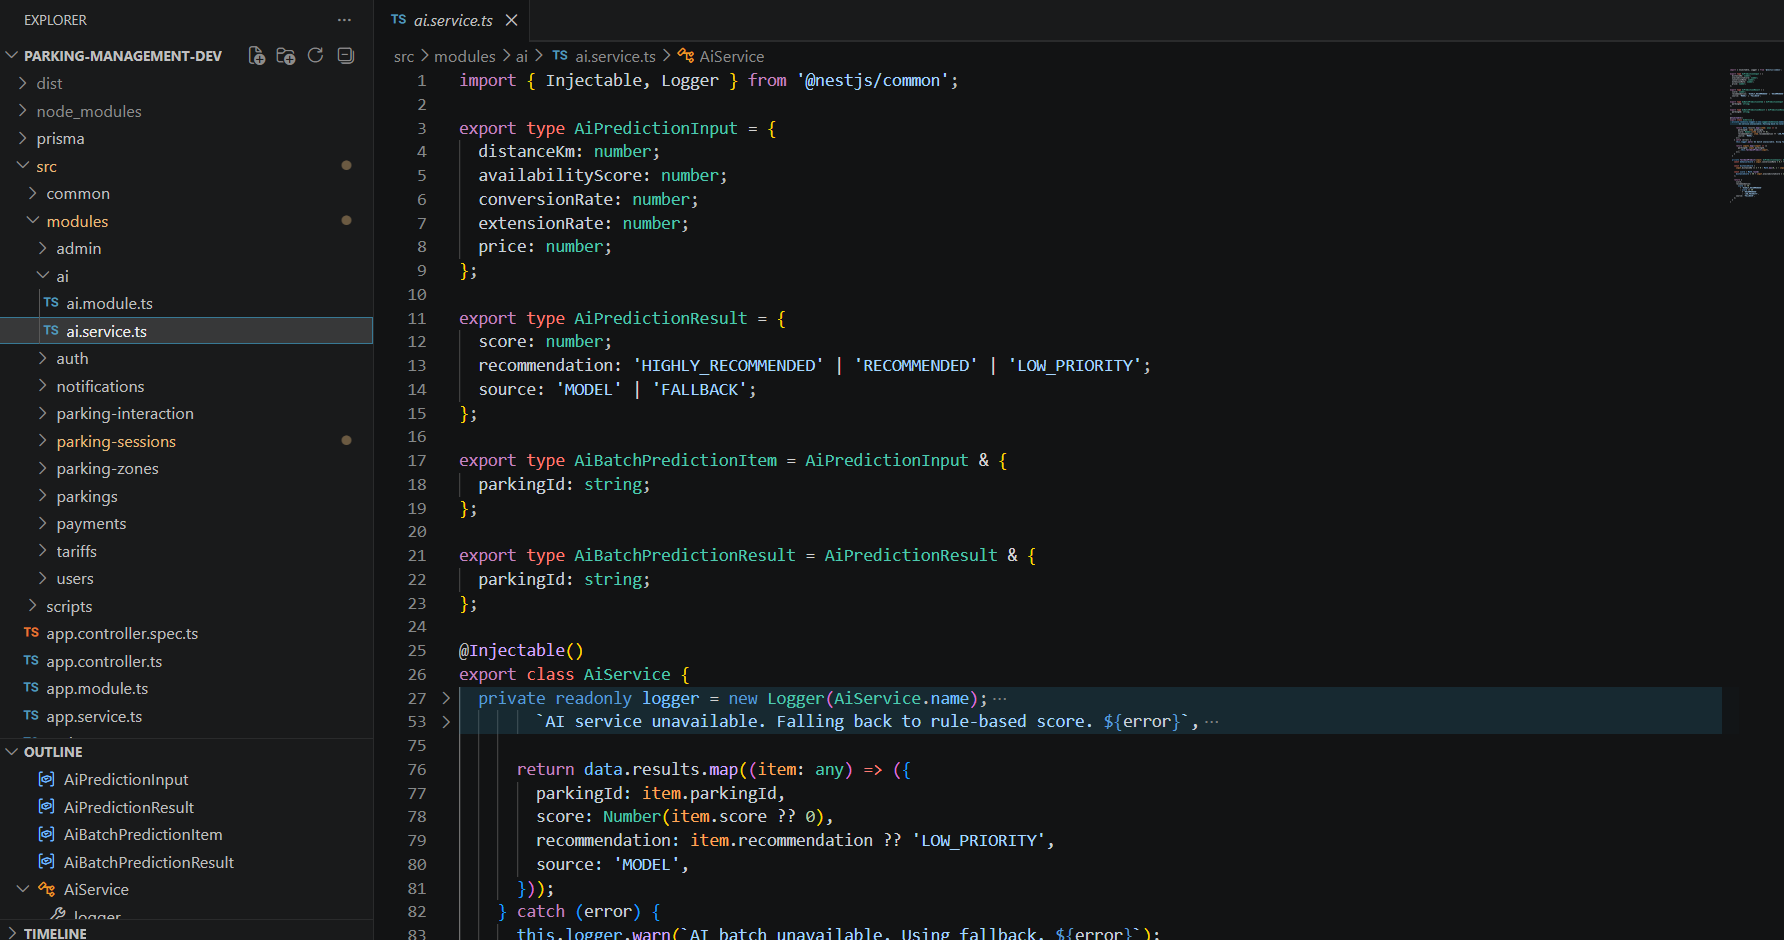
\includegraphics[width=\textwidth]{img/backend_ai.png}
    \caption{Implémentation du module de recommandation intelligente}
    \label{fig:backend_ai}
\end{figure}
\subsection{Module de notifications}

\par Le module de notifications informe les utilisateurs des événements importants de l'application, tels que la validation d'un parking privé, la confirmation d'un paiement ou l'activation d'une session de stationnement.

\par Les notifications sont enregistrées dans la base de données et transmises aux appareils mobiles grâce à \textbf{Firebase Cloud Messaging}. Les jetons FCM des utilisateurs sont également gérés par ce module afin d'assurer la distribution des notifications Push.

\begin{figure}[H]
    \centering
    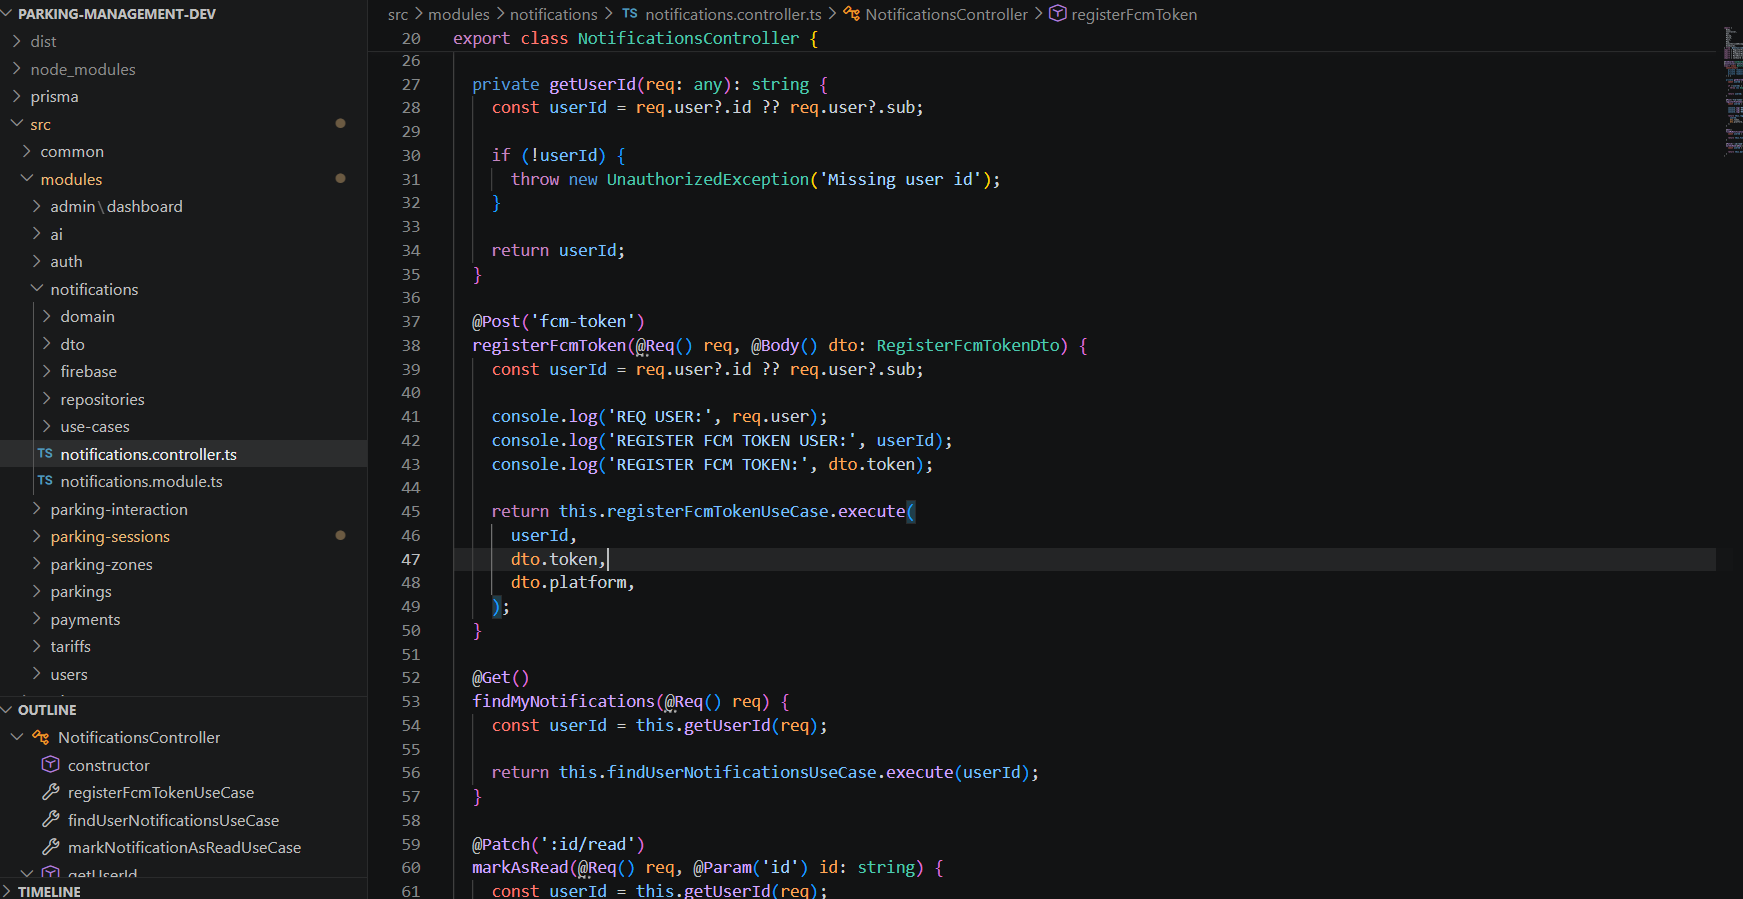
\includegraphics[width=\textwidth]{img/backend_notification.png}
    \caption{Implémentation du module de notifications}
    \label{fig:backend_notification}
\end{figure}

\subsection{Module des interactions avec les parkings}

\par Le module des interactions enregistre les différentes actions réalisées par les utilisateurs sur les parkings. Chaque consultation d'un parking, démarrage de session ou prolongation de stationnement est enregistrée dans la base de données.

\par Ces informations permettent de produire des statistiques d'utilisation et sont exploitées par le système de recommandation intelligent afin d'évaluer la popularité des parkings et d'améliorer la pertinence des recommandations proposées aux utilisateurs.

\begin{figure}[H]
    \centering
    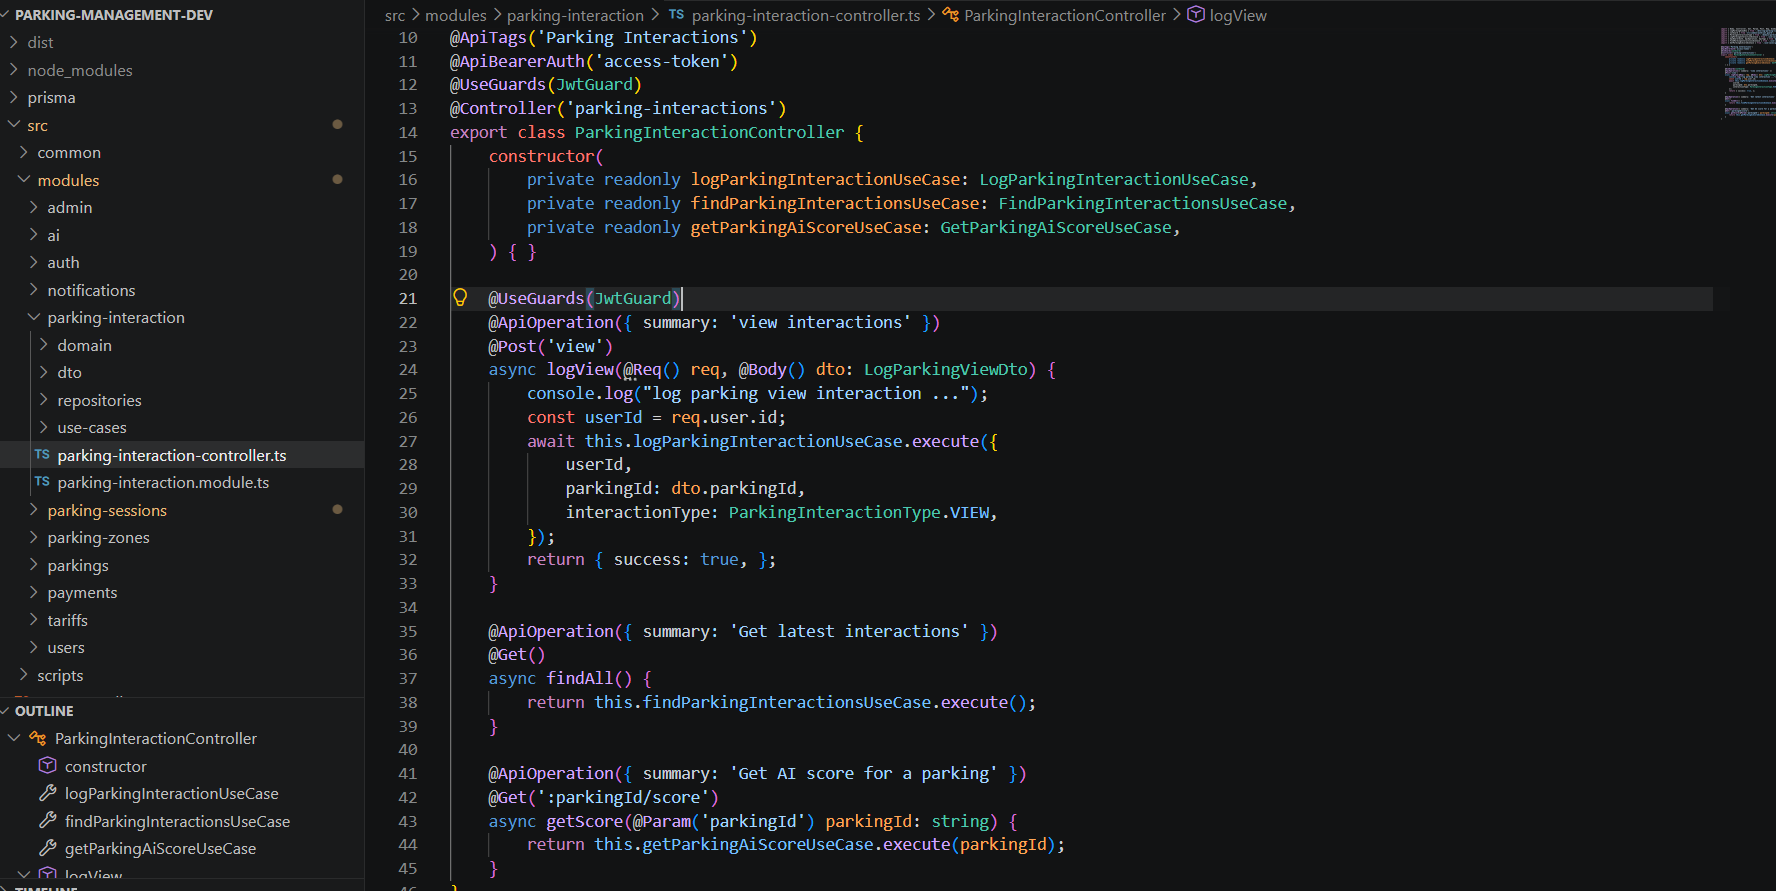
\includegraphics[width=\textwidth]{img/backend_interaction.png}
    \caption{Implémentation du module des interactions avec les parkings}
    \label{fig:backend_interaction}
\end{figure}


\subsection{Module de gestion des utilisateurs}

\par Ce module permet de gérer les comptes des utilisateurs de la plateforme. Il prend en charge la création des comptes, la mise à jour des informations personnelles, la gestion des rôles ainsi que la vérification des adresses électroniques et des numéros de téléphone.

\par Le module assure également l'administration des comptes, notamment le blocage d'un utilisateur, la récupération du mot de passe et la gestion des différents profils tels que les utilisateurs, les propriétaires de parkings, les auditeurs et les administrateurs.

\begin{figure}[H]
    \centering
    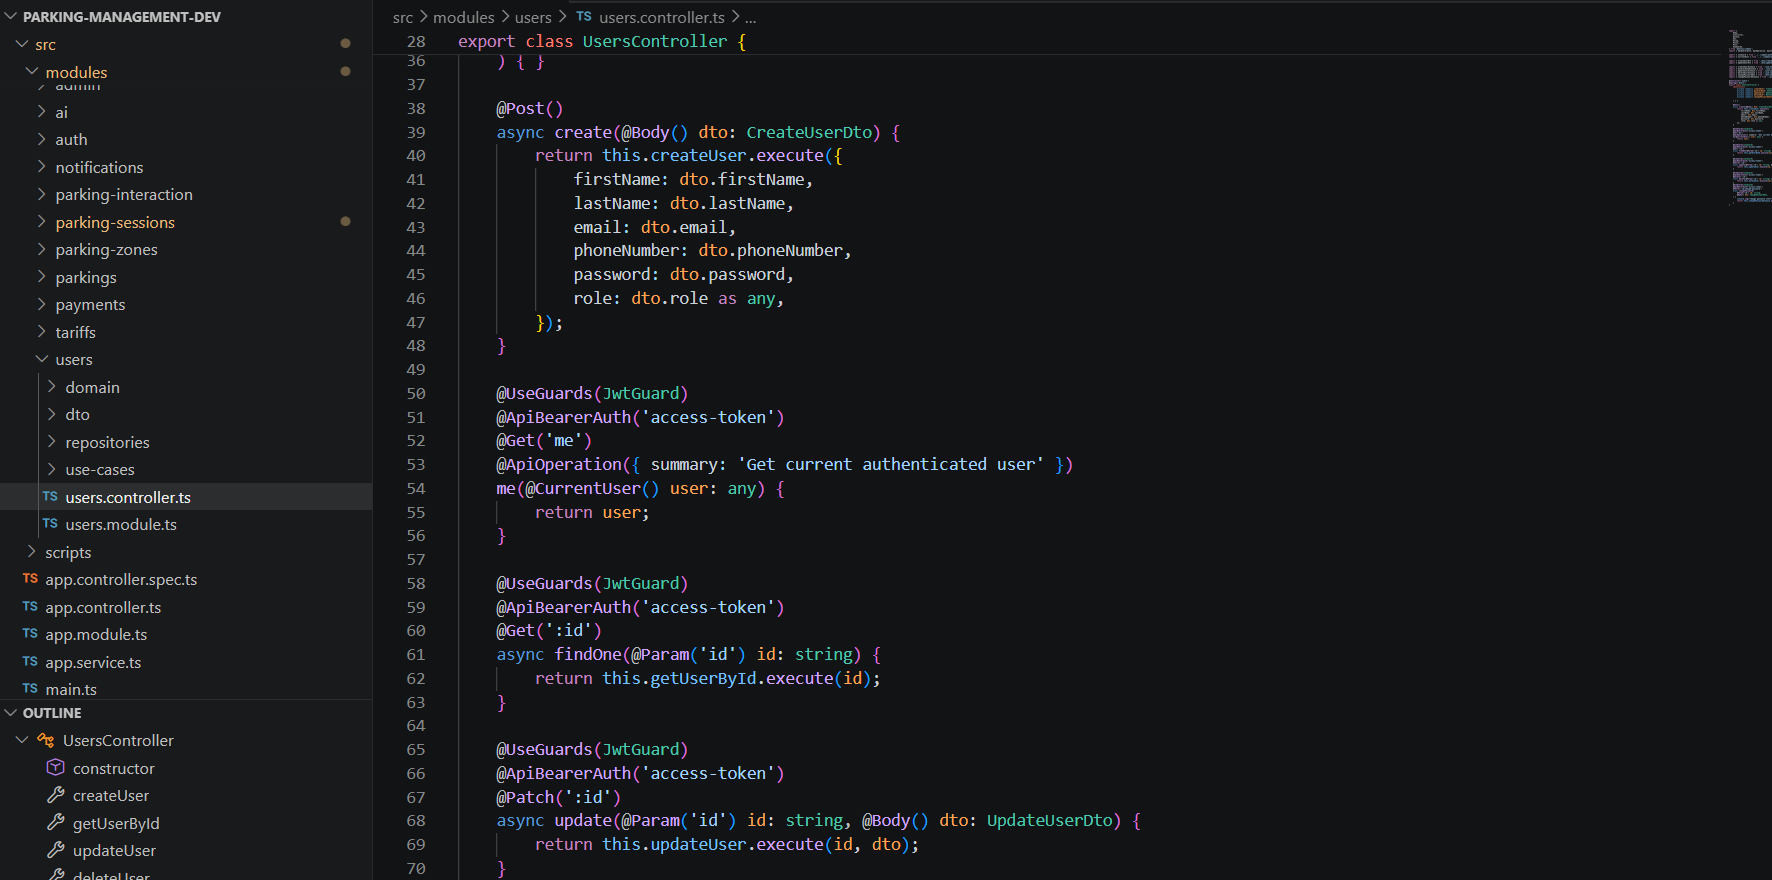
\includegraphics[width=\textwidth]{img/backend_user.png}
    \caption{Implémentation du module de gestion des utilisateurs}
    \label{fig:backend_user}
\end{figure}



\section{Implémentation de l'application mobile}

\par \textbf{TuniPark} a été développée à l'aide du framework \textbf{Flutter}. Elle permet aux utilisateurs de rechercher des parkings, de gérer leurs sessions de stationnement, d'effectuer des paiements sécurisés et de consulter leur historique. L'application adopte une architecture modulaire reposant sur le principe du \textit{Clean Architecture}, ce qui facilite la maintenance, les évolutions futures et la réutilisation du code.

\par Les interfaces ont été conçues afin d'offrir une navigation simple et intuitive tout en exploitant les fonctionnalités natives du smartphone, notamment la géolocalisation, les notifications Push et le stockage sécurisé des informations d'authentification.


\subsection{Authentification}

\par Ces interfaces permettent aux utilisateurs de créer un compte, de se connecter et de récupérer leur mot de passe. La plateforme prend en charge l'authentification par adresse électronique ou numéro de téléphone. En cas d'oubli du mot de passe, un code OTP est envoyé afin de vérifier l'identité de l'utilisateur avant de lui permettre de définir un nouveau mot de passe.

\begin{figure}[H]
    \centering
    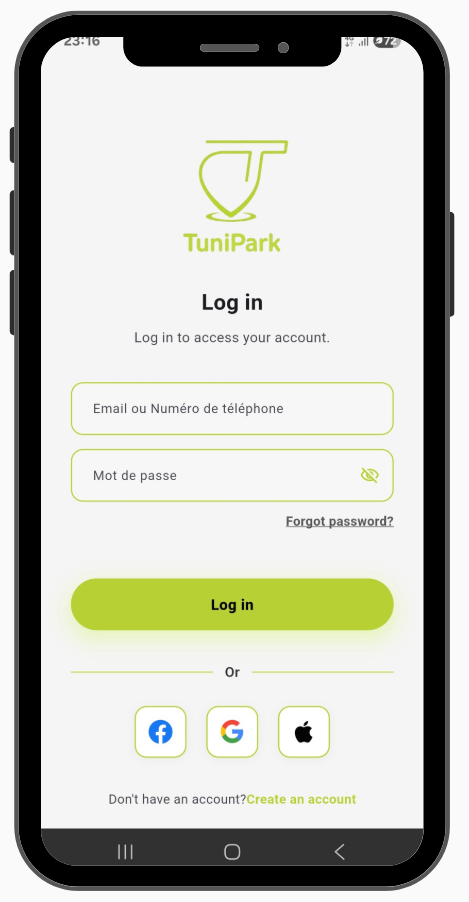
\includegraphics[width=0.5\textwidth]{img/auth_screens.png}
    \caption{Interfaces d'authentification}
    \label{fig:auth_screens}
\end{figure}

\subsection{Exploration des parkings}

\par Après authentification, l'utilisateur accède à la page d'exploration. Celle-ci affiche les parkings disponibles à proximité sous forme de carte interactive accompagnée de recommandations générées par le système intelligent. L'utilisateur a la possibilité de visualiser les détails de chaque parking avant de démarrer une session.

\begin{figure}[H]
    \centering
    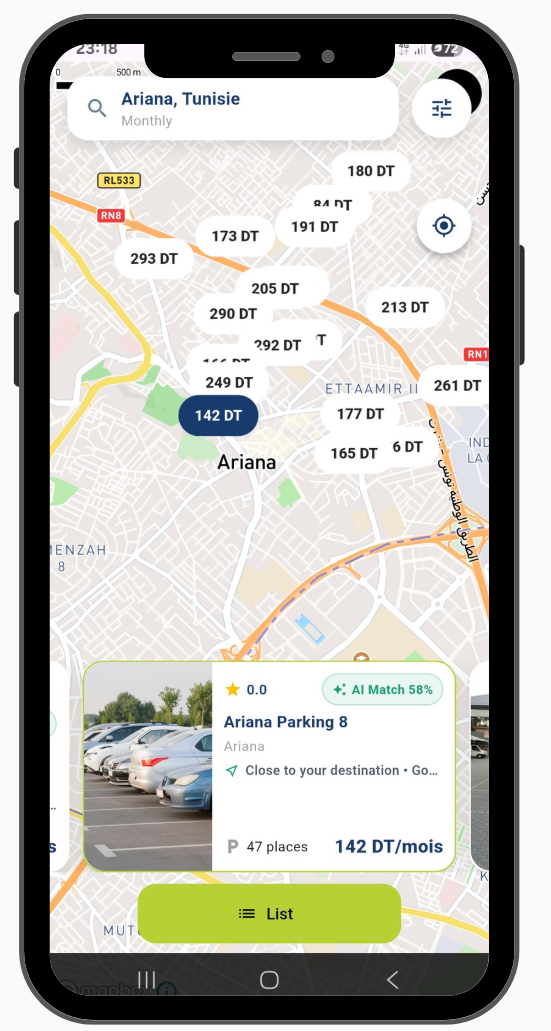
\includegraphics[width=0.5\textwidth]{img/explore_screens.png}
    \caption{Exploration des parkings}
    \label{fig:explore}
\end{figure}

\subsection{Création d'une session de stationnement}

\par Pour démarrer une session de stationnement, l'utilisateur sélectionne un parking puis renseigne les informations nécessaires concernant son véhicule et la durée souhaitée. Une fois les informations validées, l'application lance automatiquement le processus de paiement.

\begin{figure}[H]
    \centering
    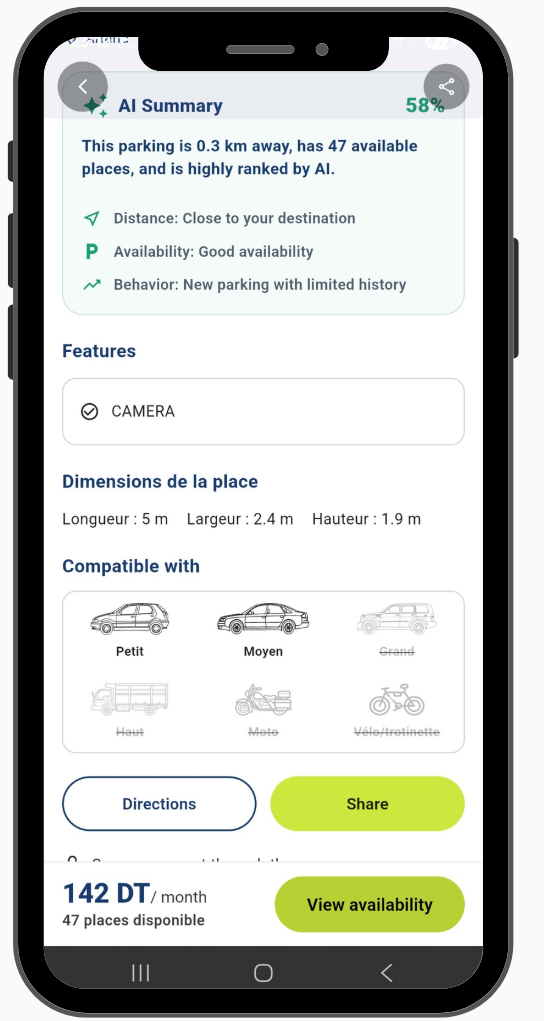
\includegraphics[width=0.5\textwidth]{img/session_creation.png}
    \caption{Création d'une session de stationnement}
    \label{fig:create_session}
\end{figure}

\subsection{Paiement d'une session}

\par Les paiements sont réalisés via la plateforme Flouci. Après validation de la transaction, l'application reçoit la confirmation du Backend et active automatiquement la session de stationnement.

\begin{figure}[H]
    \centering
    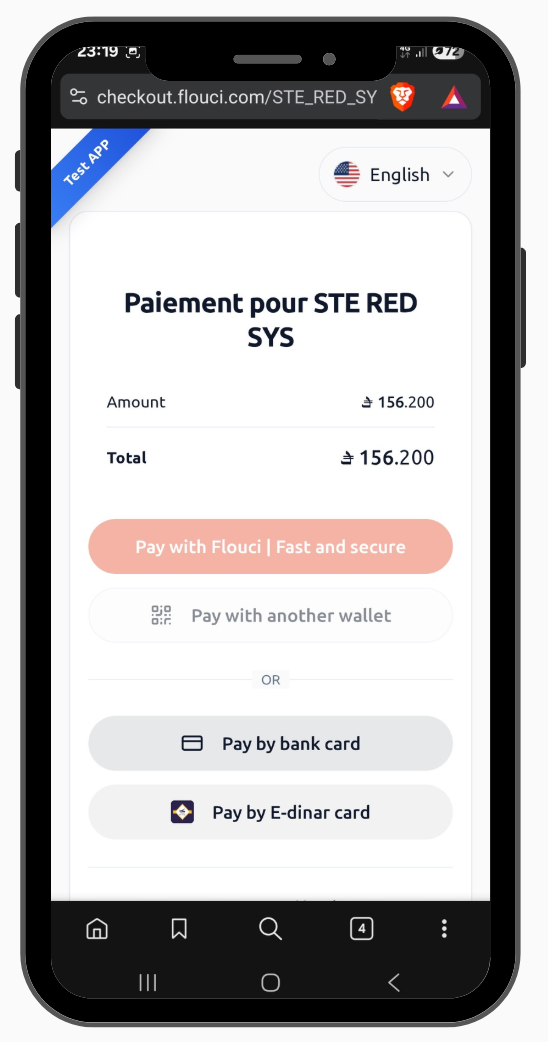
\includegraphics[width=.5\textwidth]{img/payment_screens.png}
    \caption{Paiement d'une session}
    \label{fig:payment}
\end{figure}

\subsection{Suivi de la session}

\par Une fois le paiement confirmé, l'usager a la possibilité de visualiser les détails concernant sa session actuelle, notamment le parking sélectionné, la durée restante et les différentes actions disponibles telles que la prolongation ou l'arrêt de la session.

\begin{figure}[H]
    \centering
    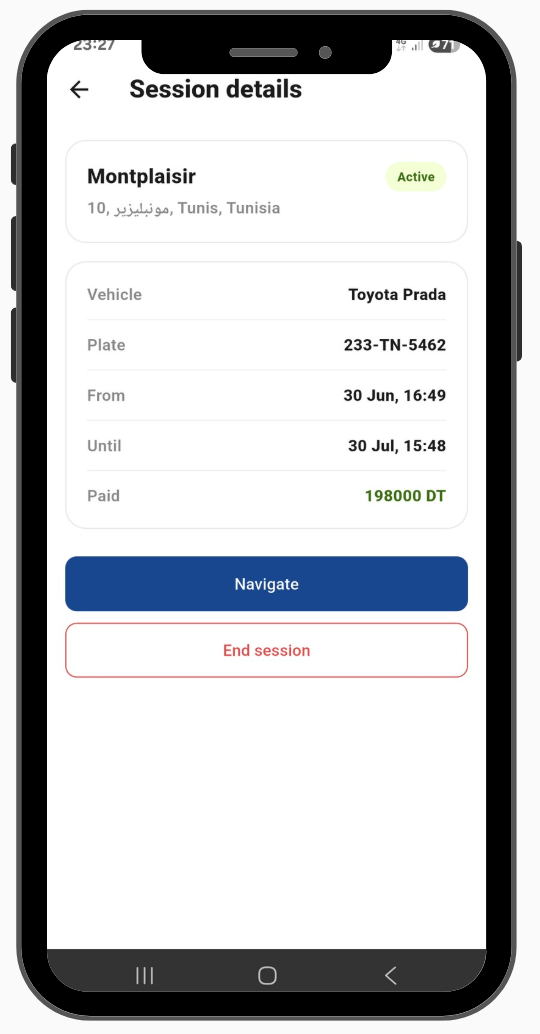
\includegraphics[width=.5\textwidth]{img/session_active.png}
    \caption{Suivi d'une session active}
    \label{fig:active_session}
\end{figure}

\subsection{Ajout d'un parking privé}

\par Les propriétaires peuvent proposer un parking privé en renseignant les informations générales, les caractéristiques, les tarifs et les photographies du parking. Après soumission, la demande est transmise à l'administrateur pour validation.

\begin{figure}[H]
    \centering
    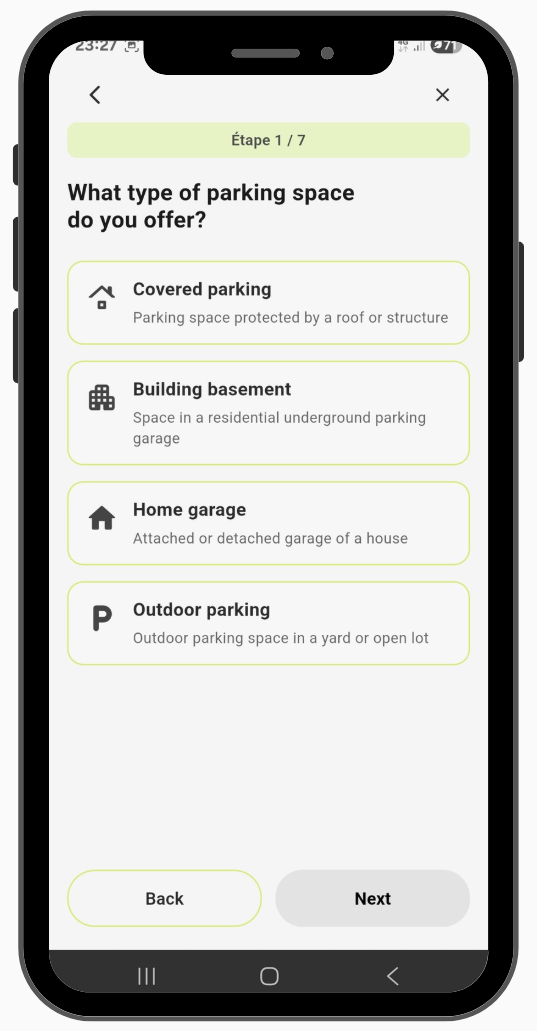
\includegraphics[width=.5\textwidth]{img/private_parking.png}
    \caption{Ajout d'un parking privé}
    \label{fig:private_parking}
\end{figure}
\subsection{Profil utilisateur}

\par L'application permet aux utilisateurs de consulter et de modifier leurs informations personnelles, de gérer leurs véhicules enregistrés ainsi que d'accéder à leur historique de stationnement.

\begin{figure}[H]
    \centering
    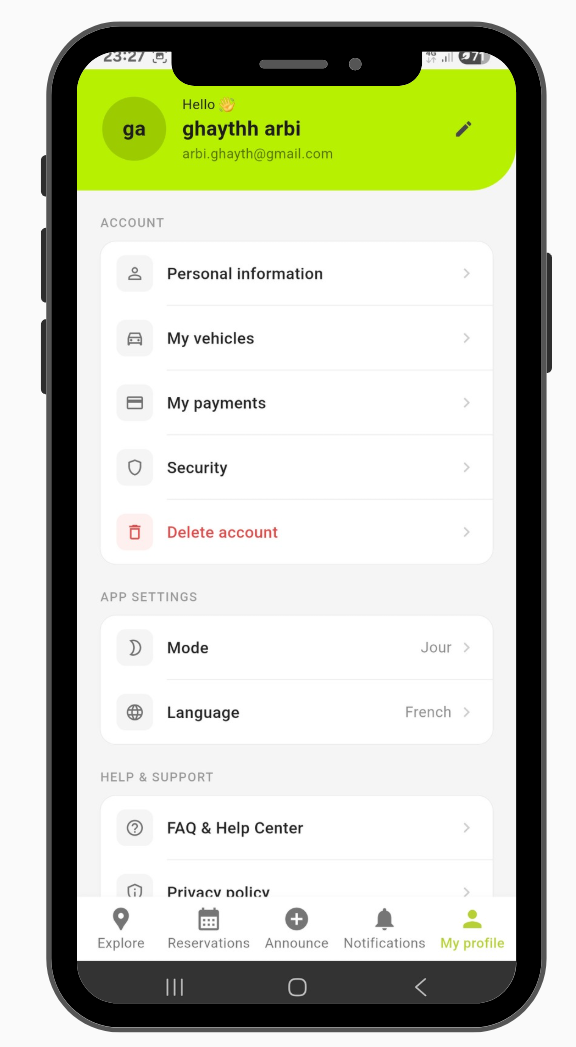
\includegraphics[width=.5\textwidth]{img/profile.png}
    \caption{Interface du profil utilisateur}
    \label{fig:profile}
\end{figure}

\subsection{Notifications}

\par Les notifications permettent d'informer l'utilisateur des événements importants de l'application, notamment la validation d'un parking privé, la confirmation d'un paiement, le début d'une session ou encore les rappels liés au stationnement.

\begin{figure}[H]
    \centering
    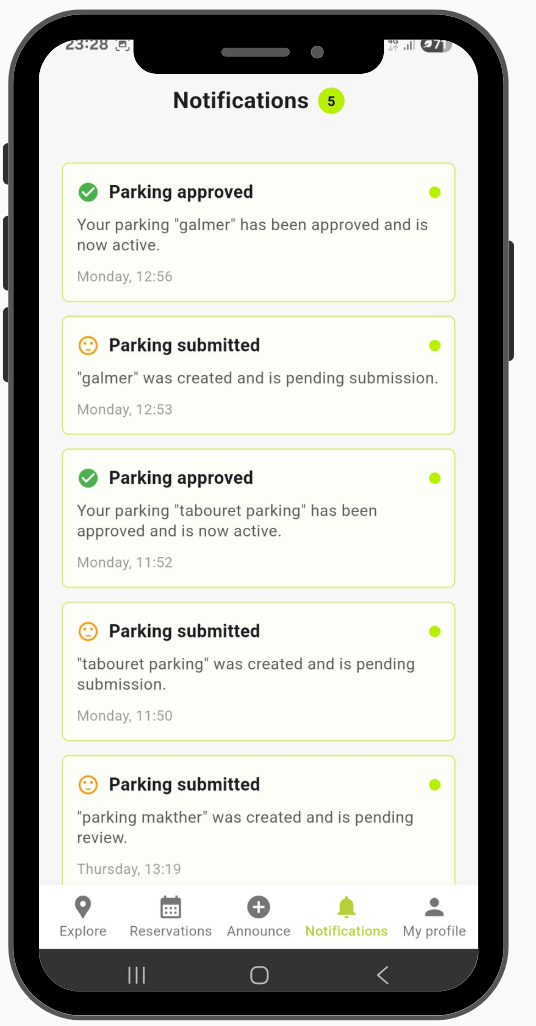
\includegraphics[width=.45\textwidth]{img/notifications.png}
    \caption{Interface des notifications}
    \label{fig:notifications}
\end{figure}
\section{Fonctionnalités administratives}

\par La plateforme web d'administration a été développée avec \textbf{Angular}. Elle est exclusivement accessible aux utilisateurs disposant des privilèges administratifs. Après authentification, l'administrateur accède à un tableau de bord lui permettant de superviser les principales opérations de l'application TuniPark.

\par L'interface d'administration centralise la gestion des utilisateurs, des parkings publics et privés, des zones de stationnement, des sessions, des paiements ainsi que des notifications. Elle permet également de valider ou refuser les requêtes d'ajout de parkings privés, de consulter les statistiques d'utilisation de la plateforme et de gérer les informations nécessaires au bon fonctionnement du système.

\begin{figure}[H]
    \centering
    \begin{minipage}{0.8\textwidth}
        \centering
        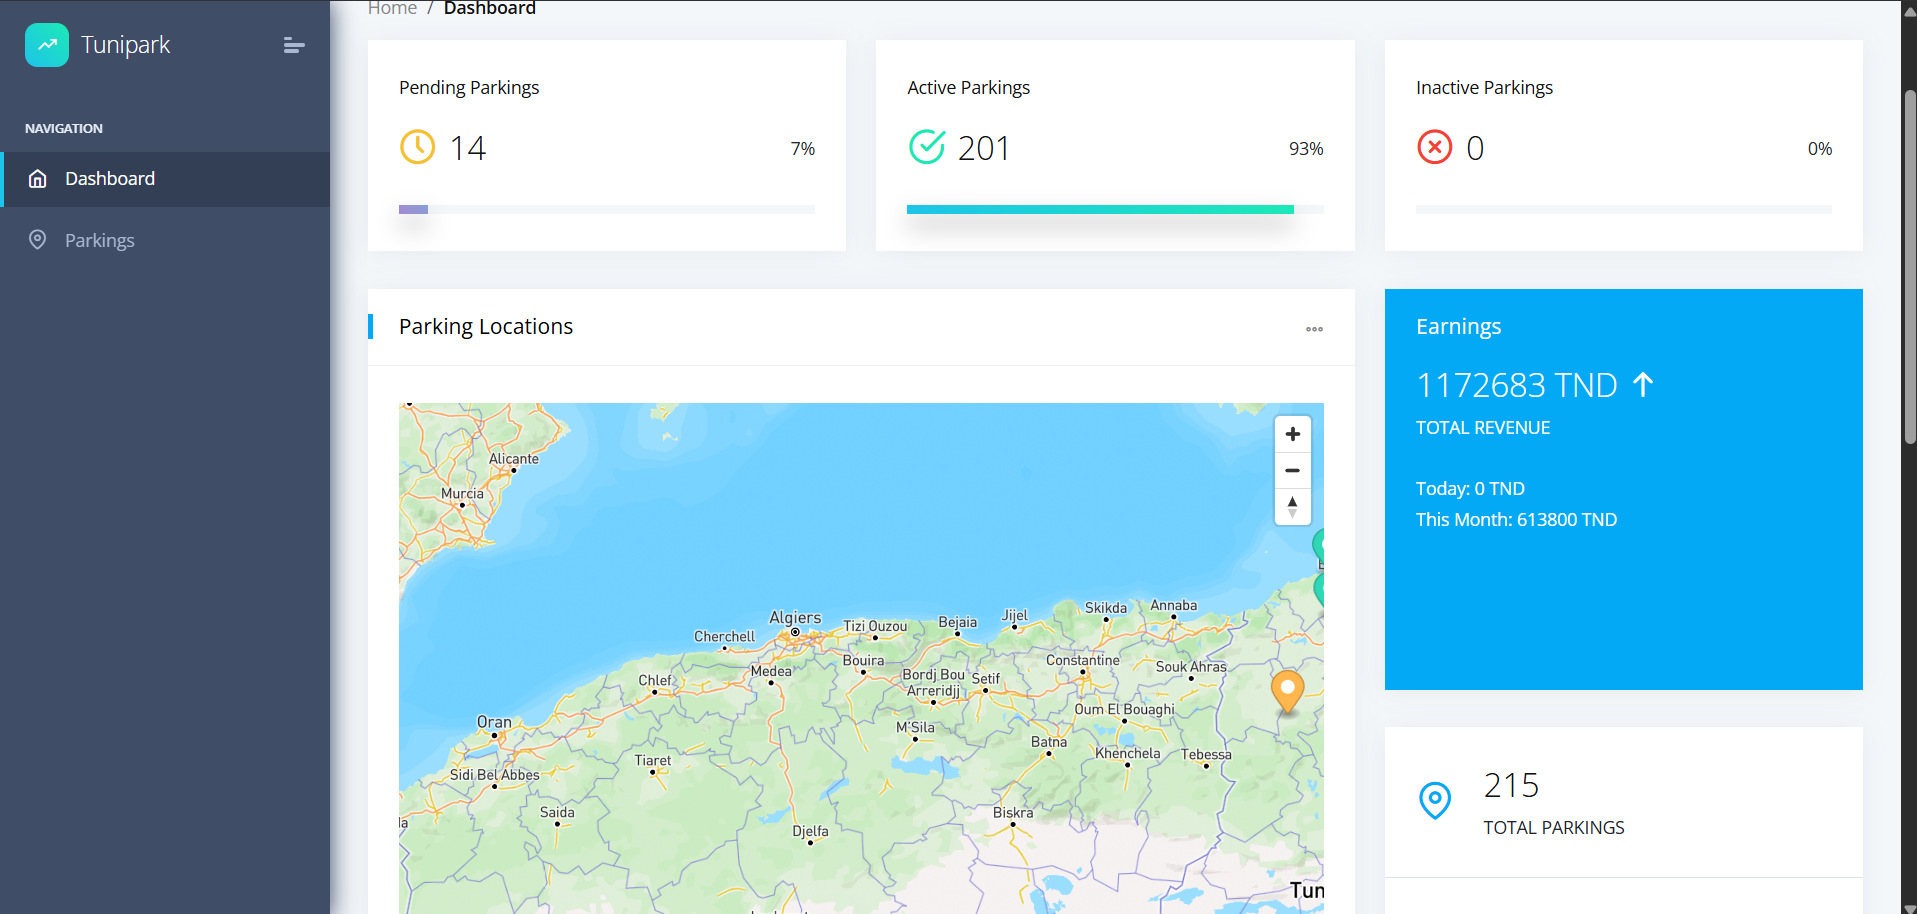
\includegraphics[width=0.95\textwidth]{img/admin_dashboard.png}
        \caption{Tableau de bord de l'administration}
        \label{fig:admin_dashboard}
    \end{minipage}
    \vfill
    \begin{minipage}{0.8\textwidth}
        \centering
        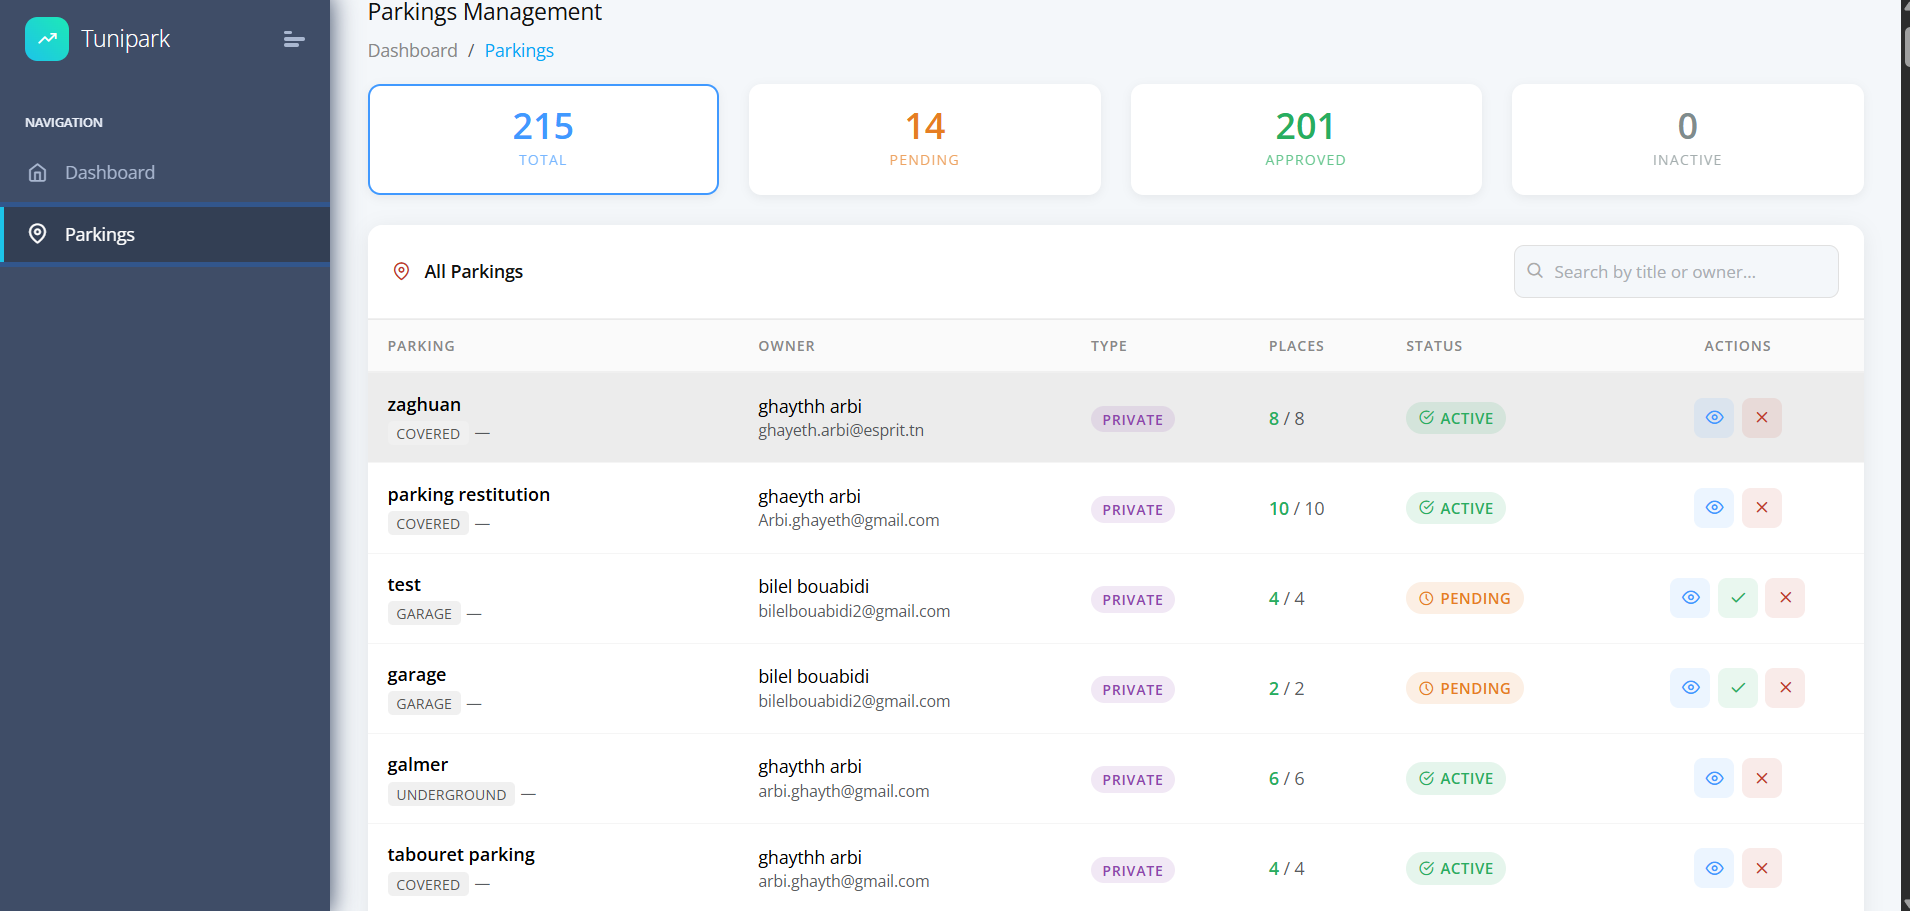
\includegraphics[width=0.95\textwidth]{img/admin_management.png}
        \caption{Interface de gestion des ressources}
        \label{fig:admin_management}
    \end{minipage}
\end{figure}
\section{Présentation du déploiement}

\par Après le développement et la validation des différentes fonctionnalités, l'application \textbf{TuniPark} a été déployée dans un context de production afin de permettre son utilisation dans des conditions réelles. Les différents composants de la plateforme sont hébergés sur des services cloud adaptés à leur rôle, garantissant leur disponibilité, leur maintenance et leur évolutivité.

\par Le Backend développé avec \textbf{NestJS} est hébergé sur la plateforme \textbf{Render}. Cette plateforme assure l'exécution continue de l'API REST ainsi que la communication avec la base de données \textbf{PostgreSQL}, également hébergée sur Render. Cette configuration permet au Backend de traiter les requêtes provenant de l'application mobile et de la plateforme web d'administration de manière sécurisée.

\begin{figure}[H]
    \centering
    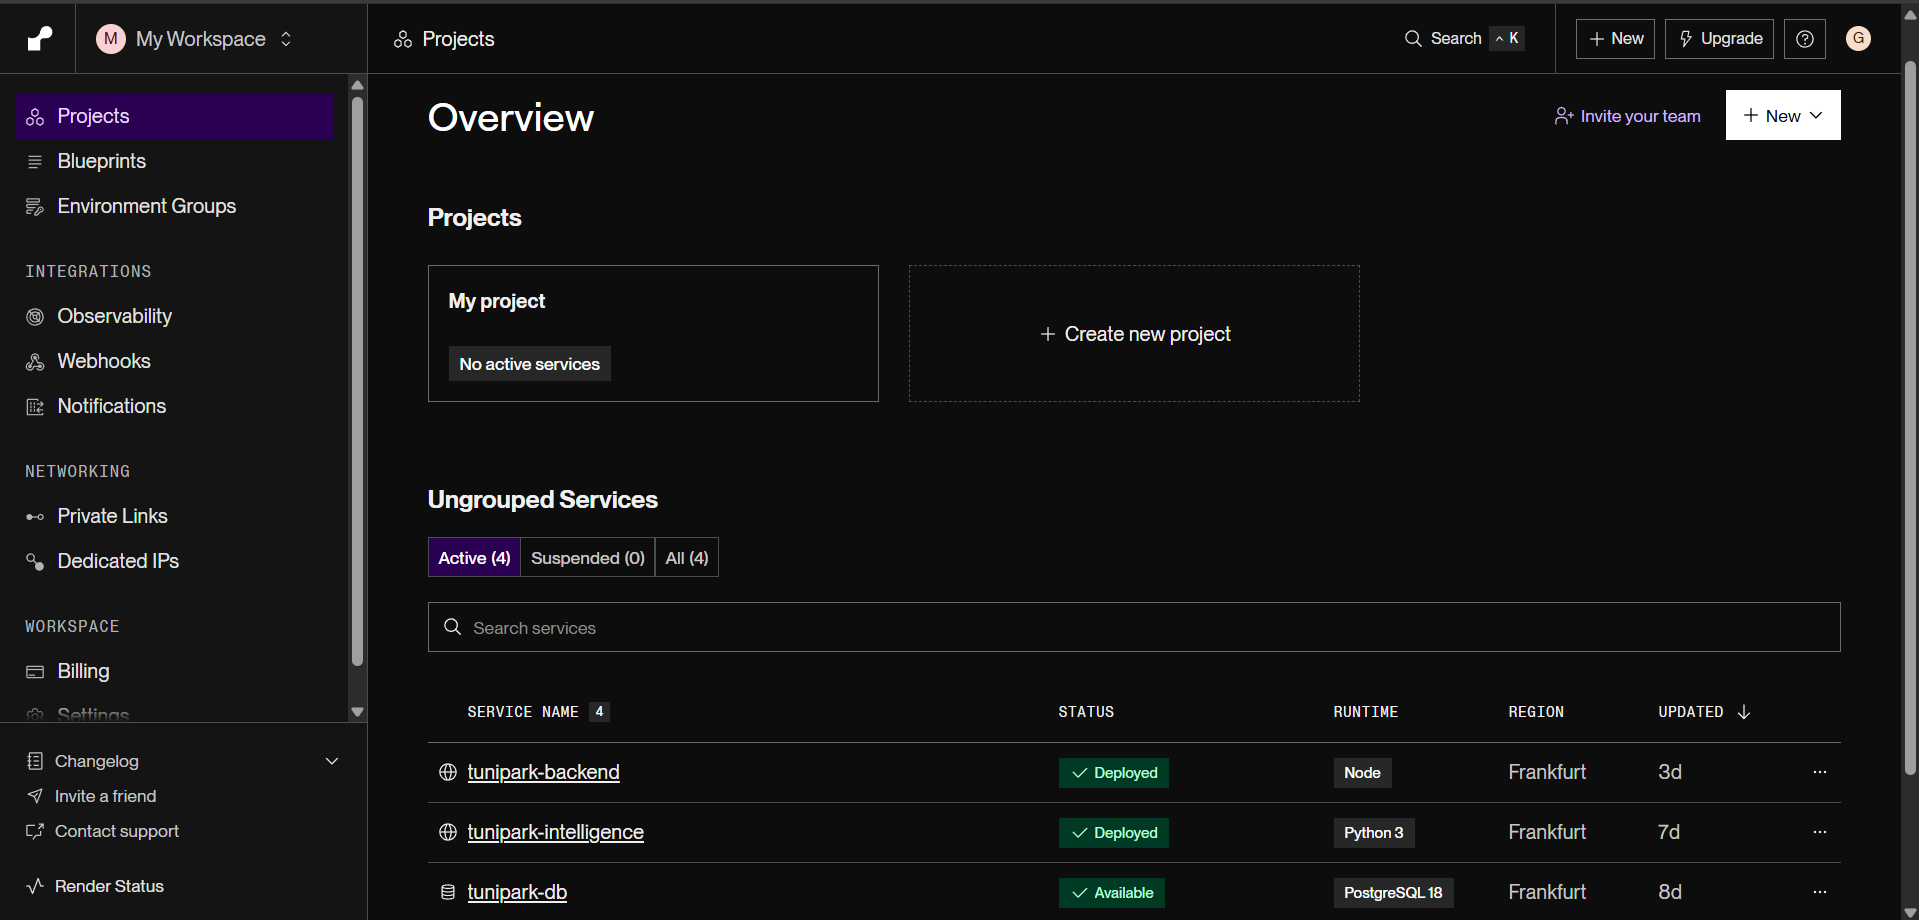
\includegraphics[width=0.95\textwidth]{img/render_dashboard.png}
    \caption{Déploiement du Backend et de la base de données sur Render}
    \label{fig:render_dashboard}
\end{figure}

\par La plateforme web d'administration développée avec \textbf{Angular} est déployée sur \textbf{Vercel}. Cette solution facilite le déploiement continu de l'application et permet la publication rapide des nouvelles versions de l'interface d'administration.

\begin{figure}[H]
    \centering
    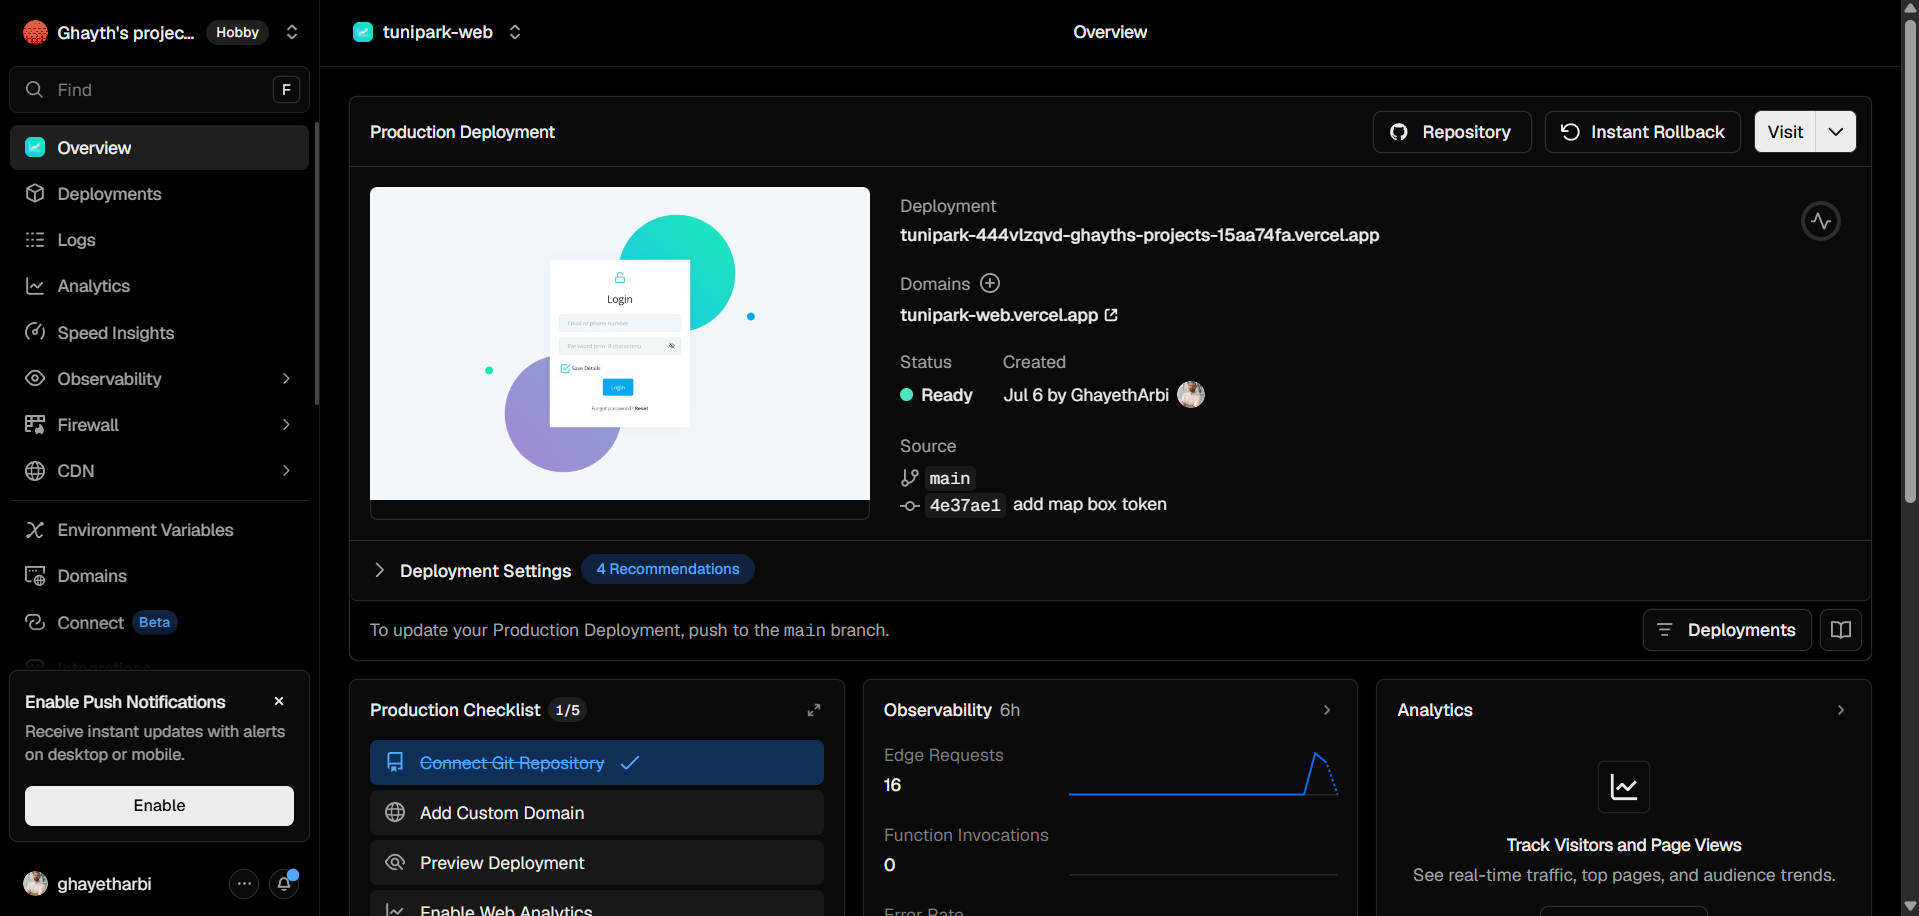
\includegraphics[width=0.95\textwidth]{img/vercel_dashboard.png}
    \caption{Déploiement de la plateforme web d'administration sur Vercel}
    \label{fig:vercel_dashboard}
\end{figure}

\par En complément de ces services, plusieurs solutions externes ont été intégrées pour garantir le fonctionnement optimal de l'application. Les images des parkings sont stockées sur \textbf{Cloudinary}, les notifications Push sont envoyées grâce à \textbf{Firebase Cloud Messaging}, les paiements électroniques sont traités par \textbf{Flouci} et les courriers électroniques sont transmis à l'aide de \textbf{Nodemailer}. L'envoi des codes OTP par SMS a été prévu via \textbf{Twilio}, mais cette fonctionnalité n'a pas été activée durant la période du projet en raison de l'absence d'un abonnement au service.

\par Cette infrastructure de déploiement permet aux différents composants de fonctionner de manière indépendante tout en garantissant une communication sécurisée entre l'application mobile, la plateforme web d'administration, le Backend, la base de données ainsi que les différents services externes intégrés à la solution.
\section{Conclusion}

\par Ce chapitre a présenté la réalisation de l'application \textbf{TuniPark} en décrivant l'environnement de développement, les principaux modules du Backend, les interfaces de l'application mobile ainsi que la plateforme web d'administration.

\par Il a également présenté les différentes fonctionnalités implémentées, notamment l'authentification sécurisée, la gestion des parkings, les sessions de stationnement, les paiements électroniques, les notifications Push et le système de recommandation intelligent basé sur un modèle Random Forest.

\par Enfin, le chapitre a décrit l'architecture de déploiement de la solution en mettant en évidence l'intégration des différents services cloud utilisés durant le projet. Le prochain chapitre portera sur tests et sur la validation de l'application afin d'évaluer son bon fonctionnement et de vérifier que les exigences définies au cours de l'analyse ont été satisfaites.